\section{Development/Implementation View}

\subsection{Component Diagram}

Biểu đồ thành phần (Component diagram) mô tả cấu trúc tổng thể của hệ thống phần mềm quản lý bãi đỗ xe thông minh (Smart Parking System). Hệ thống được tổ chức thành nhiều lớp (layer) nhằm đảm bảo tính phân tách trách nhiệm (separation of concerns), dễ bảo trì và dễ mở rộng. Dựa vào kiến trúc phân lớp, hệ thống bao gồm 5 lớp chính:
\begin{itemize}
    \item User Interface Layer
    \item Application/Service Layer
    \item Business/Domain Layer
    \item Data Access Layer
    \item Integration Layer
\end{itemize}

% TODO: Chèn ảnh Component Diagram của bạn vào đây
\begin{figure}[H]
    \centering
    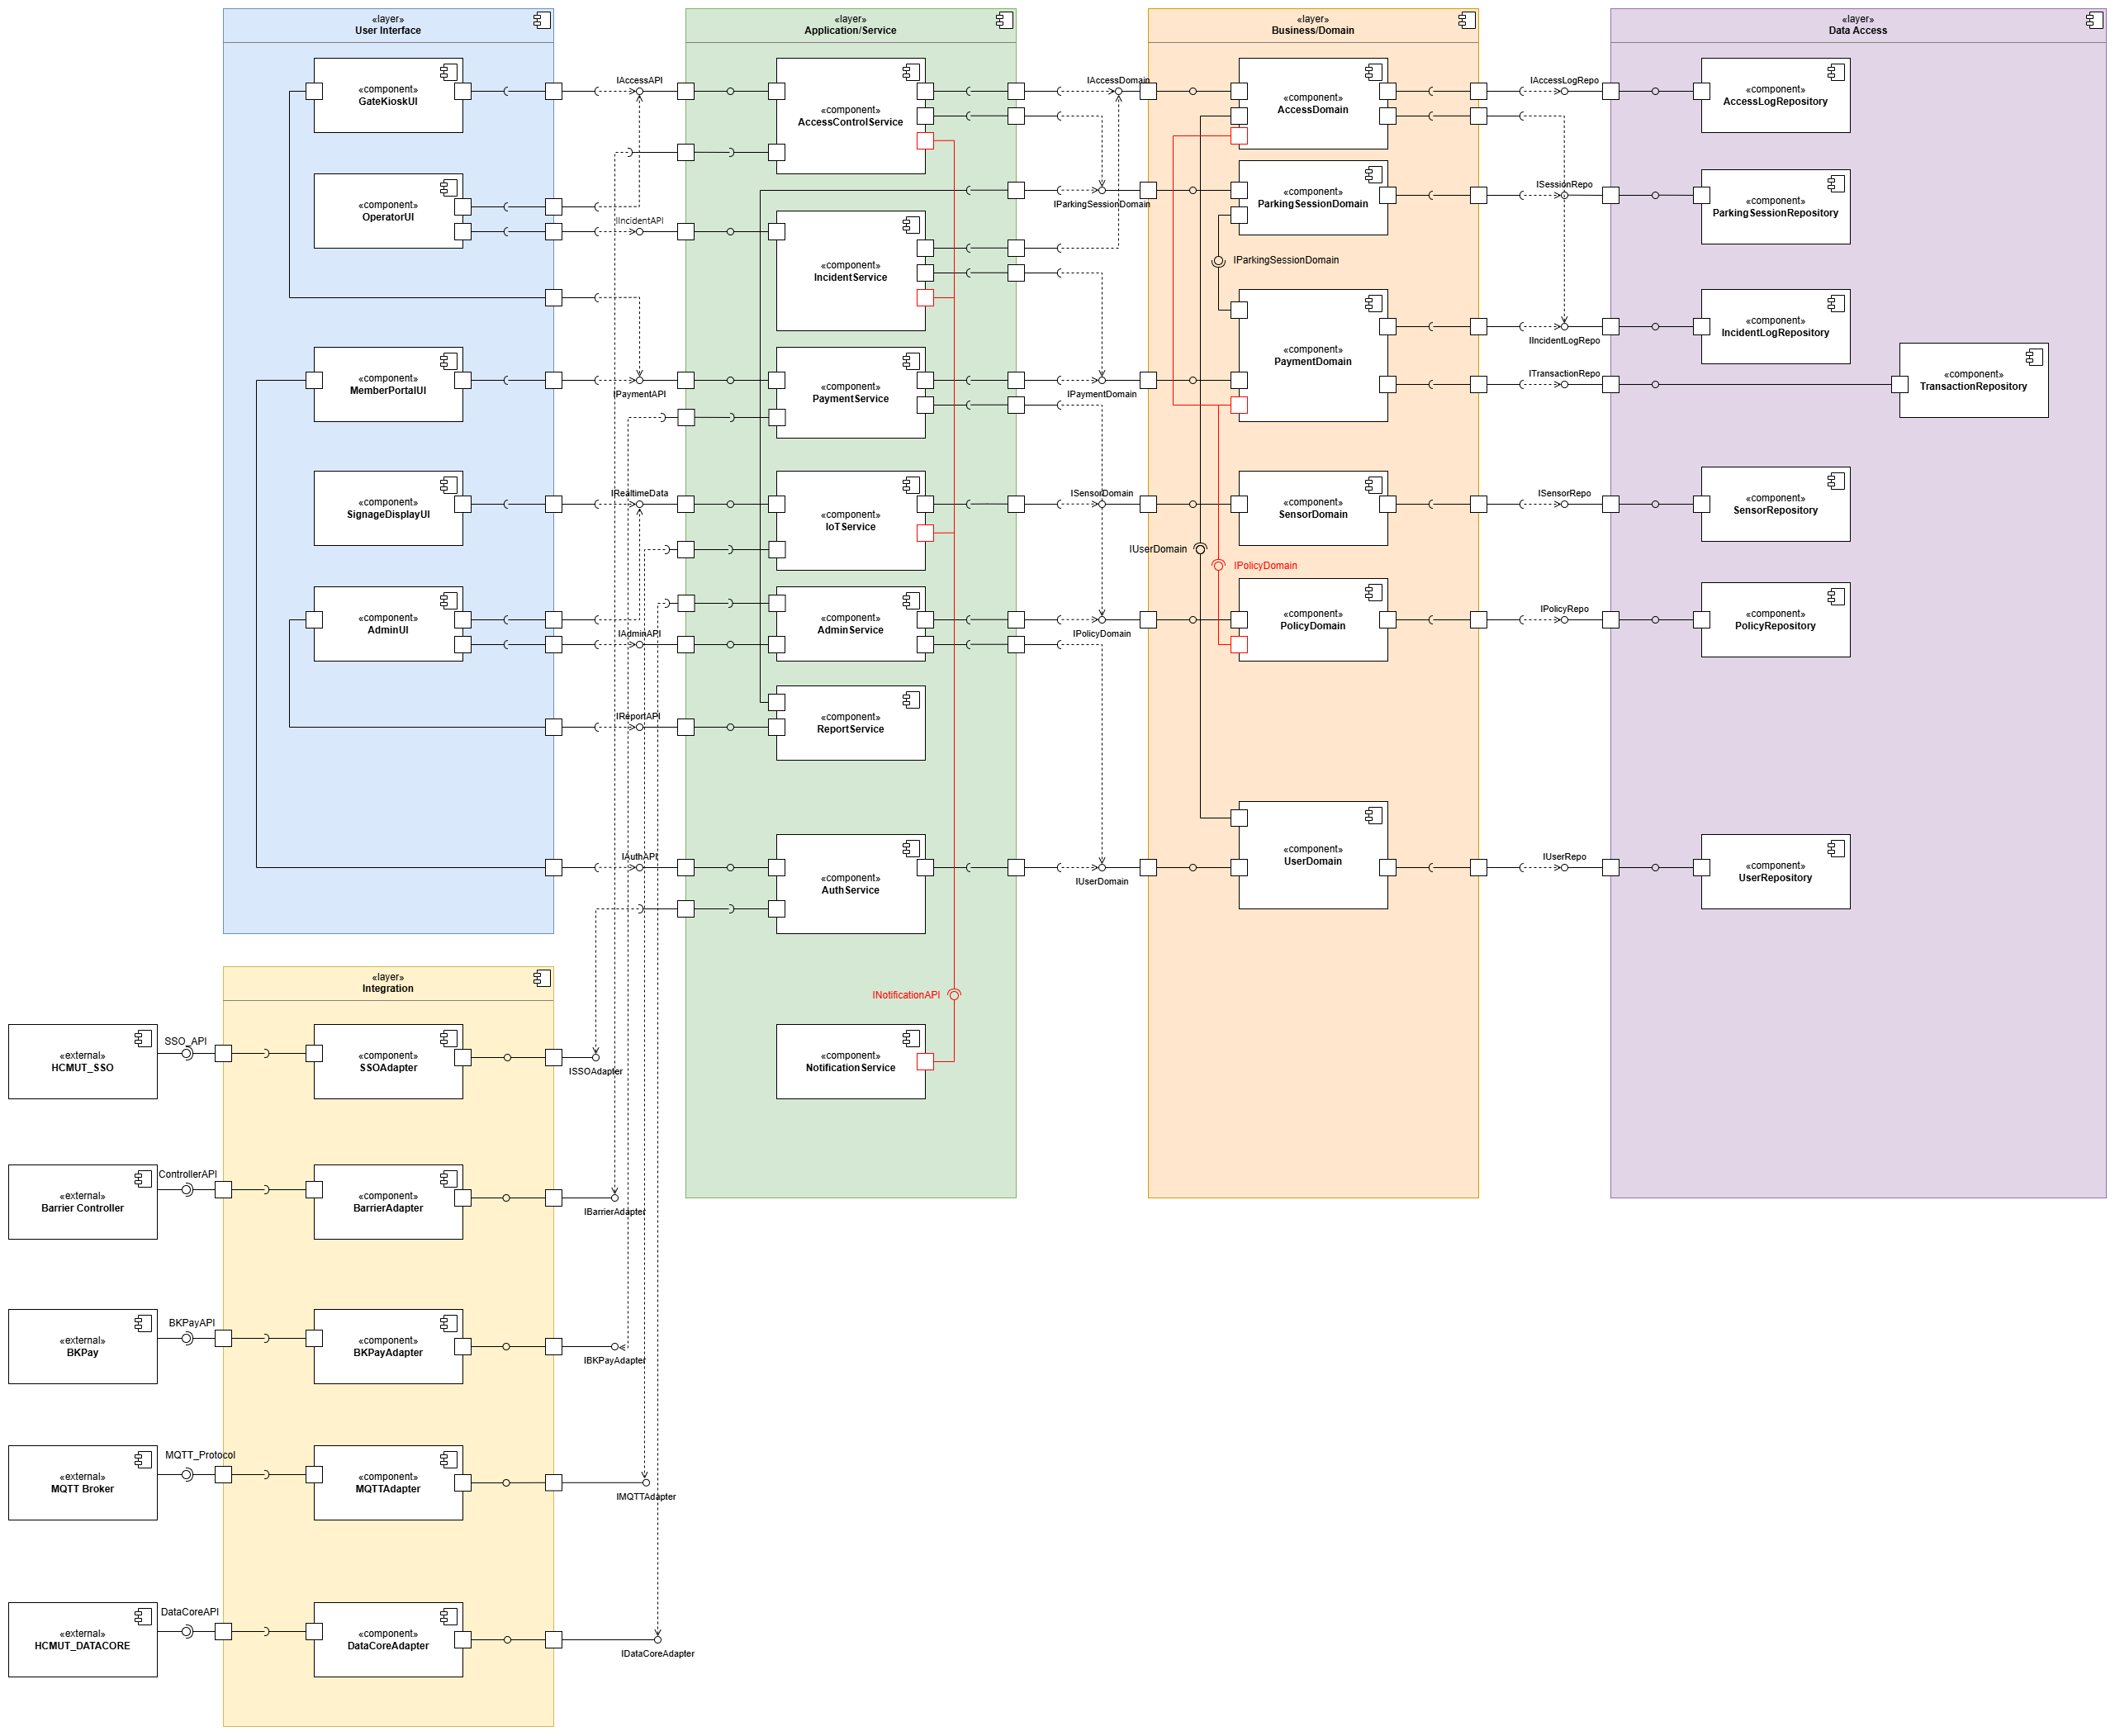
\includegraphics[origin=c, width=\textwidth, height=0.9\textheight, keepaspectratio]{../design/component_diagram.png}
    \caption{Component Diagram của hệ thống Smart Parking}
    \label{fig:component_diagram}
\end{figure}

\subsubsection{User Interface Layer}
Lớp này gồm các component giao diện trực tiếp tương tác với từng nhóm người dùng hoặc thiết bị hiển thị. Các component UI không chứa logic nghiệp vụ, chúng chỉ tiếp nhận thao tác của người dùng và gọi các component trong lớp Application/Service thông qua các interface được cung cấp (ví dụ: \texttt{IAccessAPI}, \texttt{IPaymentAPI}, \texttt{IRealTimeData}).
\begin{itemize}
    \item \textbf{GateKioskUI:} Giao diện tại cổng rào dành cho khách vãng lai và thành viên quét thẻ/thanh toán.
    \item \textbf{OperatorUI:} Giao diện hỗ trợ nhân viên bãi xe theo dõi luồng xe và xử lý các sự cố (ví dụ: mở cổng thủ công).
    \item \textbf{MemberPortalUI:} Giao diện dành cho người dùng nội bộ (sinh viên, cán bộ) quản lý thông tin, gia hạn gói gửi xe.
    \item \textbf{SignageDisplayUI:} Giao diện cho bảng LED điện tử hiển thị số lượng chỗ trống còn lại.
    \item \textbf{AdminUI:} Bảng điều khiển (dashboard) dành cho quản trị viên cấu hình hệ thống, quản lý chính sách và xem báo cáo.
\end{itemize}

\subsubsection{Application/Service Layer}
Đây là lớp triển khai các use-case của hệ thống. Mỗi component đại diện cho một nhóm chức năng điều phối nghiệp vụ, xử lý luồng (workflow), kiểm tra dữ liệu đầu vào và gọi lớp Business/Domain để thực hiện logic cốt lõi. Lớp này cũng giao tiếp với hệ thống bên ngoài thông qua Integration Layer. Các component chính gồm:
\begin{itemize}
    \item \textbf{AccessControlService:} Điều phối quy trình vào/ra bãi xe, xác thực thẻ và ra lệnh điều khiển barrier.
    \item \textbf{IncidentService:} Xử lý các luồng sự cố bất thường và ghi nhận log sự kiện.
    \item \textbf{PaymentService:} Điều phối quy trình thanh toán vé vãng lai hoặc gia hạn vé tháng.
    \item \textbf{IoTService:} Thu thập và xử lý tín hiệu từ cảm biến (sensor), cập nhật trạng thái bãi xe theo thời gian thực.
    \item \textbf{AdminService:} Điều phối các thao tác quản trị hệ thống, cập nhật cấu hình và đồng bộ dữ liệu.
    \item \textbf{ReportService:} Truy xuất và tổng hợp dữ liệu thống kê.
    \item \textbf{AuthService:} Điều phối quy trình đăng nhập, phân quyền người dùng.
    \item \textbf{NotificationService:} Cung cấp \texttt{INotificationAPI} để nhận trigger và gửi các thông báo (alert) từ các service khác.
\end{itemize}

\subsubsection{Business/Domain Layer}
Đây là lớp chứa logic nghiệp vụ cốt lõi của hệ thống. Các component biểu diễn các hành vi, quy tắc và điều kiện liên quan đến thực thể (entity) trong hệ thống:
\begin{itemize}
    \item \textbf{AccessDomain:} Định nghĩa quy tắc ra/vào, kiểm tra tính hợp lệ của thẻ từ.
    \item \textbf{ParkingSessionDomain:} Quản lý vòng đời của một phiên đỗ xe (thời gian vào, thời gian ra, vị trí).
    \item \textbf{PaymentDomain:} Xử lý các quy tắc tính toán chi phí đỗ xe theo từng loại phương tiện và người dùng.
    \item \textbf{SensorDomain:} Xử lý logic dữ liệu cảm biến thô để xác định trạng thái trống/đầy của chỗ đỗ.
    \item \textbf{PolicyDomain:} Quản lý các quy định, chính sách về giá cả và phân loại người dùng (được tham chiếu thông qua \texttt{IPolicyDomain}).
    \item \textbf{UserDomain:} Chứa các logic liên quan đến thông tin và trạng thái (khóa/mở) của người dùng.
\end{itemize}

\subsubsection{Data Access Layer}
Lớp này cung cấp các giao diện trừu tượng để truy cập dữ liệu liên tục trong hệ thống. Mỗi repository quản lý các thao tác truy xuất đối với một nhóm thực thể trong Database.
\begin{itemize}
    \item \textbf{AccessLogRepository:} Lưu trữ và truy xuất lịch sử ra/vào cổng.
    \item \textbf{ParkingSessionRepository:} Lưu trữ các phiên gửi xe đang hoạt động và đã kết thúc.
    \item \textbf{IncidentLogRepository:} Ghi chép lịch sử xử lý sự cố tại bãi xe.
    \item \textbf{TransactionRepository:} Quản lý lịch sử giao dịch và biên lai thanh toán.
    \item \textbf{SensorRepository:} Lưu trữ trạng thái cấu hình và lịch sử dữ liệu của các cảm biến IoT.
    \item \textbf{PolicyRepository:} Quản lý dữ liệu cài đặt chính sách giá, quy định.
    \item \textbf{UserRepository:} Lưu trữ thông tin tài khoản và thẻ từ của người dùng.
\end{itemize}

\subsubsection{Integration Layer}
Lớp này đóng vai trò là một ranh giới cách ly (anti-corruption layer), chứa các Adapter dùng để kết nối với những hệ thống bên ngoài (\texttt{<<external>>}). Việc sử dụng Adapter đảm bảo hệ thống nội bộ không bị ảnh hưởng khi API bên ngoài thay đổi.
\begin{itemize}
    \item \textbf{SSOAdapter:} Giao tiếp với \texttt{HCMUT\_SSO} thông qua \texttt{SSO\_API} để xác thực đăng nhập.
    \item \textbf{BarrierAdapter:} Giao tiếp với bộ điều khiển phần cứng \texttt{Barrier Controller} thông qua \texttt{ControllerAPI} để thực thi lệnh đóng/mở cổng.
    \item \textbf{BKPayAdapter:} Giao tiếp với cổng thanh toán \texttt{BKPay} thông qua \texttt{BKPayAPI} để tạo yêu cầu và xác nhận thanh toán.
    \item \textbf{MQTTAdapter:} Giao tiếp với \texttt{MQTT Broker} qua \texttt{MQTT\_Protocol} để thu thập bản tin từ gateway cảm biến.
    \item \textbf{DataCoreAdapter:} Giao tiếp với \texttt{HCMUT\_DATACORE} qua \texttt{DataCoreAPI} để đồng bộ thông tin sinh viên, cán bộ.
\end{itemize}

\subsection{Implementation Frameworks}
\begin{itemize}
    \item \textbf{Frontend Framework:} Next.js (React), TypeScript, Tailwind CSS
    \item \textbf{State Management \textsl{\&} Simulated Backend:} Zustand, React Context (Client-side mock database)
    \item \textbf{Data Visualization:} Recharts
\end{itemize}
